Finally we have benchmarked \eko{} comparing to other PDFs by means of \lhapdf{}.
In \cref{fig:Hera_ct18_bench} we report a comparison of the evolution of
HERAPDF20 and CT18 at \nnlo{} from $\mu_{F}^2=\mu_{0}^2 \rightarrow 10^4~GeV$, where
$Q_{0}$ is the relative fitting scale.

During the fitting procedure two PDFs sets are evolved from the fitting scales
with different tools: respectively \hoppet{} and \qcdnum{}, while both collaborations used
\xfitter{} as a minimizer.

The benchmark with respect to HERAPDF20 indicates an agreement with \eko{}
both for singlet and valence-like quantities with a relative accuracy of $\mathcal{O}(10^{-3})$.
On the other hand the comparison with CT18 is more subtle and some discrepancies are visible
in the low-x region for valence-like quantities. We remark that even in this where the relative accuracy
deteriorate quickly, the absolute difference remains under control so the benchmark can be considered
acceptable.

\gmerror{Do we want to keep this benchmark?? Expand explanation ?}

\begin{figure}
      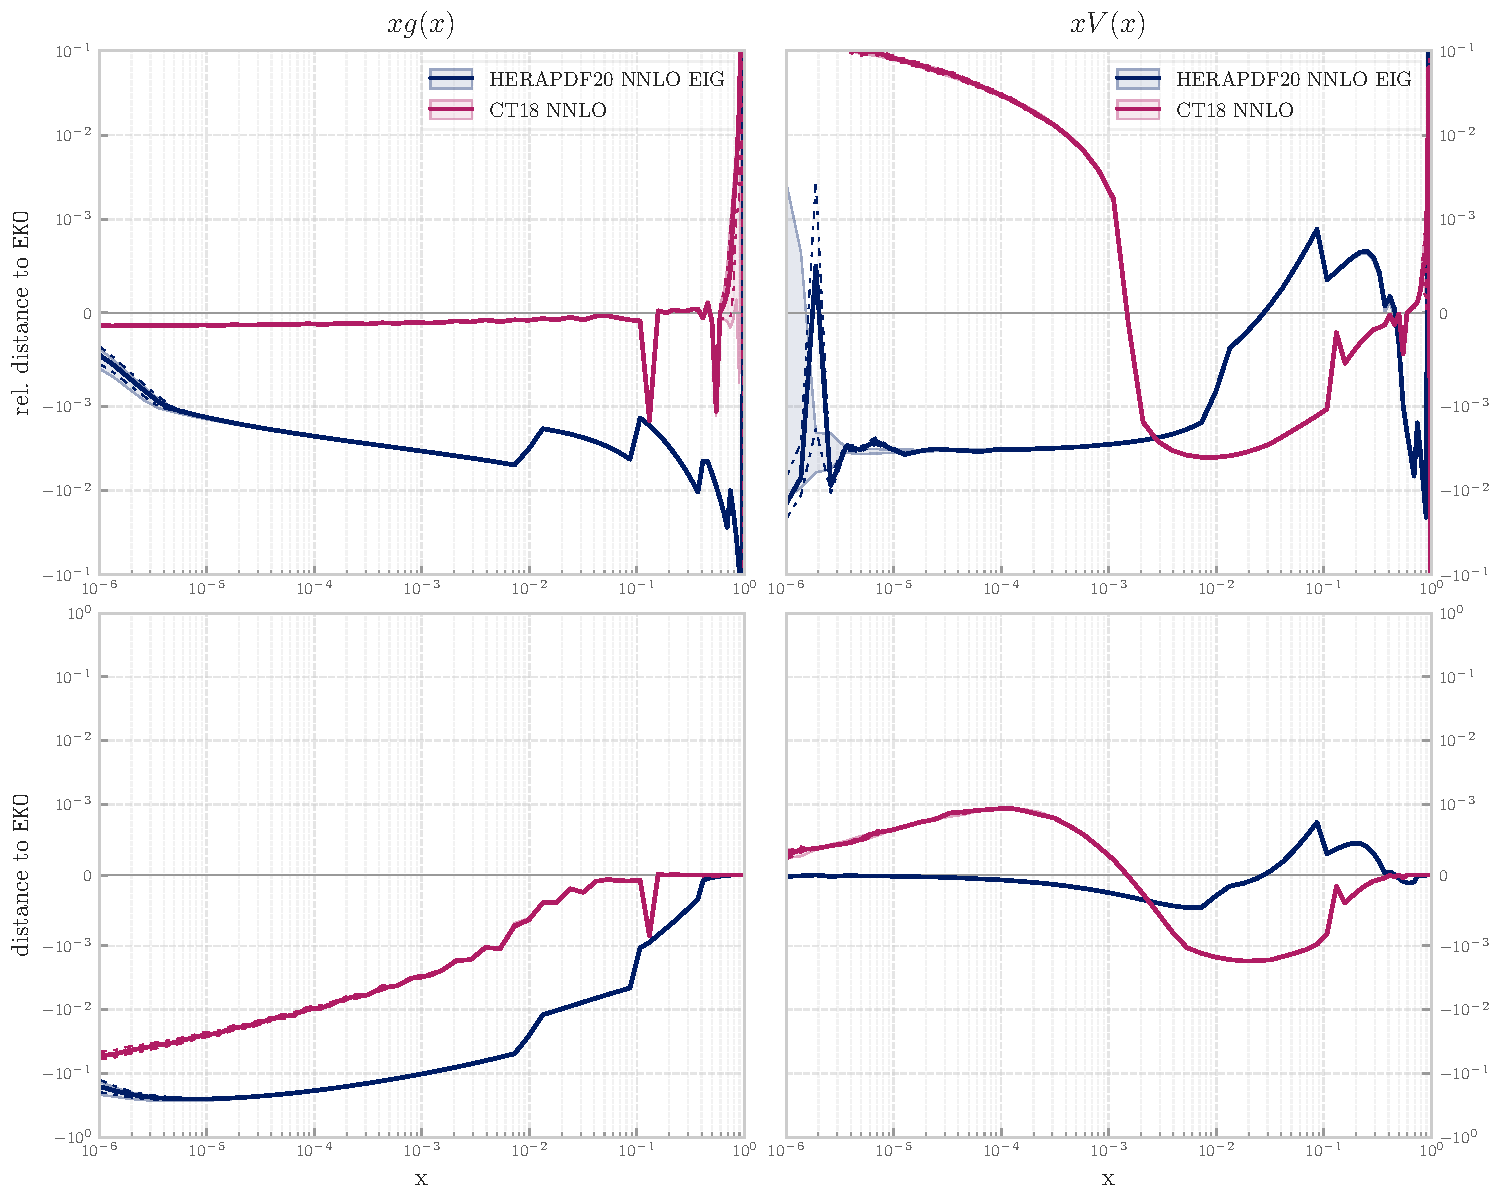
\includegraphics[width=\linewidth]{ch-eko/hera_ct18_bench.pdf}
      \caption{Relative (top)  and absolute (bottom) differences between
          the outcome of \nnlo{} \qcd{} evolution
          as implemented in \eko{} and the
          corresponding results from \lhapdf{} for HERAPDF20 and CT18.
          The evolution range is taken from the fitting scale to $\mu_{F}^2=10^4~GeV$.
          \label{fig:Hera_ct18_bench} }
  \end{figure}
